 \section{Experimental Results}
 \label{section:experiment}
In this section, we evaluate our proposed approach and present the results of applying our methods to various images. 
Our experiments were conducted on several images from \cite{draa2014artificial} and additional images (color, grayscale, and text) sourced from the Internet. 
Building on previous works in image enhancement~\cite{draa2014artificial, bhandari2020cuckoo, samanta2018log} and to conduct a comprehensive evaluation, we experimented with a total of 18 images. 
For color images, we convert them to the HSV format and change the contrast in the image by manipulating brightness without affecting the color. 
However, we observed that our proposed method performs particularly well on grayscale images. 
% For color images, we convert them to the HSV format and change the contrast in the image by manipulating brightness without affecting the color. 
Therefore, we present the results specifically for grayscale images ($13$ images).
Our experiment study reveals that the genetic algorithm with $(P,P)$ strategy outperforms the genetic algorithm with $(P+P)$ strategy. Thus, we present the results of genetic algorithm with $(P,P)$ strategy.
In the further analysis, we consider the technique:
\begin{enumerate}
  \item (HC) Hill Climbing (Subsection \ref{subsection:method_hc})
  \item (GA) Genetic Algorithm with $(P, P)$ strategy (Subsection \ref{subsection:method_ga})
\end{enumerate}
\subsection{Experimental Setup and Environment}
To evaluate the efficacy of our approach, we implemented a prototype in Python using the DEAP evolutionary computation framework\footnote{\url{https://deap.readthedocs.io/en/master/}}. For the fuzzy logic component, we utilized the scikit-fuzzy toolbox\footnote{\url{https://pythonhosted.org/scikit-fuzzy/}}.
All variants of our algorithms were executed on a system with an Intel(R) Core(TM) i$3$ CPU M$370$ @ $2.40$GHz processor, $6$GB RAM, running Ubuntu $18.04$, and Python version $3.6.8$.
% will be available after acceptance
% Our experiment code can be found in this link, \href{https://dicta2024.dictaconference.org/}{redacted for review version}.
\subsection{Results}
\label{subsection:exp_result_result}

% We visually present outputs of $13$ grayscale and text images. 
% For the sake of extensive comparative analysis, we are confined to a relatively small number of images, which is also common among prior literature~\cite{tarawneh2020automatic,veluchamy2019image} (
Due to the space limitation, we are unable to include all the enhanced or generated images in the paper. 
We first present the attained result by pointing out changes in features of four images. 
Figures \ref{fig:jetplane_output_image_ga}, \ref{fig:07_output_image_ga}, \ref{fig:house_output_image_ga}, \ref{fig:13_output_image_ga} show output images generated by our technique against the reference input images.
As an outcome of our technique, the enhanced images are more natural looking in the case of Figures~\ref{fig:07_output_image_ga}, \ref{fig:house_output_image_ga}. In Figures \ref{fig:jetplane_output_image_ga},
\ref{fig:house_output_image_ga} and \ref{fig:13_output_image_ga} we can see the edges are sharper (notice the house shadow and roof tiles, cloud at top of jetplane and mountain body). Overall the histogram is expanded, and the contrast between the black and white portion has increased. Also, it is visually noticeable that method GA is doing better than HC. We will see support behind this claim in~\Cref{subsection:exp_result_survey}. A downside of our method is that some black portions (e.g., Figures \ref{fig:house_output_image_hc}, \ref{fig:house_output_image_ga}) are unnecessarily darkened. This can be beneficial in the case of overexposed images. For example, both methods in Figure \ref{fig:07_result} and \ref{fig:13_result} are succeeded in increasing the contrast between the person's background, face, and contrast between letters and page.

For quantitative comparisons, we compute the Michelson contrast~\cite{michelson1995studies,rizzi2004proposal}, PSNR~\cite{asamoah2018measuring}, and SSIM~\cite{WBSS2004} of each enhanced image in~\Cref{tab:image_metrics} through Hill Climbing (HC) and Genetic Algorithm (GA) variants of the proposed methods. 
We compare similar metrics with images enhanced through techniques: histogram equalization (HE),  {\em dual channel} prior-based nighttime low illumination image enhancement (Dual)~\cite{SZGZZ2018}, and adaptive gamma correction with weighting distribution (AGCWD)~\cite{HCC2012}. 

The higher value of contrast indicates better contrast by increasing the difference between the darkest and brightest pixels. The table demonstrates that our proposed methods (especially GA) are effective in image contrast enhancement in most of the images compared to the original image. HE, Dual, and AGCWD have achieved better contrast metric value. Upon visual inspection, it is revealed that these three methods manage to increase contrast by darkening the dark region and brightening the bright region. In all presented images, Dual and AGCW affect oppositely compared to our method, that is they overexpose the already bright area in the images. This explains why HE, AGCW, and Dual is doing well in the Michelson contrast metric. Another observation is that out of all $5$ methods, HE introduces noticeable artifacts (grainy feature in Figures \ref{fig:07_image_he}, \ref{fig:house_image_he}, \ref{fig:13_image_he}, \ref{fig:12_image_he}, \ref{fig:11_image_he}). This explains the lower value attained in SSIM and PSNR metrics in most of the images by HE compared to other methods. Our method consistently achieved near $1$ SSIM value (worst is $>0.7$) compared to the other three. This indicates our method will introduce fewer artifacts (grainy feature, emphasized boundary, whitened area, etc.).

We can realize that only one metric does not show all sides of improvement by the same methods. The visual quality of the image is a subjective manner. For a more complete and subjective assessment of the visual quality, we have conducted a survey on our method enhanced images which we present in the next section.


\subsection{Survey}
\label{subsection:exp_result_survey}
% \subsubsection{Variant Selection to Select Survey Images}
% First, we have grouped the variants according to used metaheuristic algorithms, namely Hill Climbing and Genetic algorithm. Then according to the method described in Subsection \ref{subsection:experiment_process}, we have ranked the variants among two groups. Based on this the selected variants from the two groups are as follows:


\subsubsection{Survey Preparation}
We have prepared an anonymous survey %\footnote{\url{https://forms.gle/9wuLKMYBShjyAaK59}} 
to get a quantitative opinion on our enhanced images. In the survey, we have placed $26$ enhanced images (produced by our technique) side-by-side with their original image. 
% The first $18$ images are from Hill Climbing with neighborhood generation with split mutation (see Section \ref{subsubsection:method_hc_traptri_split}), and the second $18$ images are the same but from the Genetic Algorithm with (P, P) strategy (see Section \ref{subsection:method_ga_join}). 
The survey participant needs to mark the enhanced image on a scale of $1-9$. As the reference, the mark of the original image was $5$; therefore, a mark of $>5$ would mean a better quality enhanced image, while $<5$ will mean image degradation. A mark of $5$ would mean the processed image is the same as the original visually (a subjective judgment). 
% The prepared survey form can be found at the following link: \href{https://dicta2024.dictaconference.org}{redacted for review version}%\url{https://forms.gle/9wuLKMYBShjyAaK59}.
%\href{https://forms.gle/9wuLKMYBShjyAaK59}{here}.

\subsubsection{Survey Response \& Observations}
We have received a total of $67$ responses. From the responses, we have filtered responses with suspicious patterns like all equal marks or very high or very low marks. This filtering caused two responses to be filtered. From the remaining $65$ responses, it seems GA, achieving a mean score of $5.45$, is better than HC, achieving a mean score $4.77$. 
Moreover, achieving a mean score of greater that $5$ indicates that the GA improves the original image.

\begin{figure}[!htb]
  \begin{subfigure}{0.23\textwidth}%
    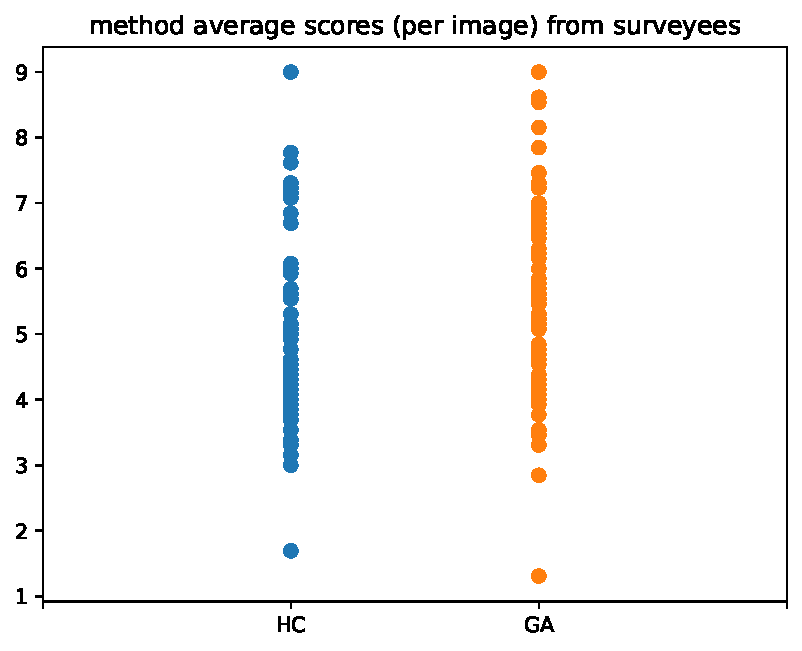
\includegraphics[width=\linewidth]{surveyee_score_scatter_plot.pdf}
    \caption{}
    \label{fig:survey_result_scatterplot}
  \end{subfigure}
\begin{subfigure}{0.23\textwidth}%
  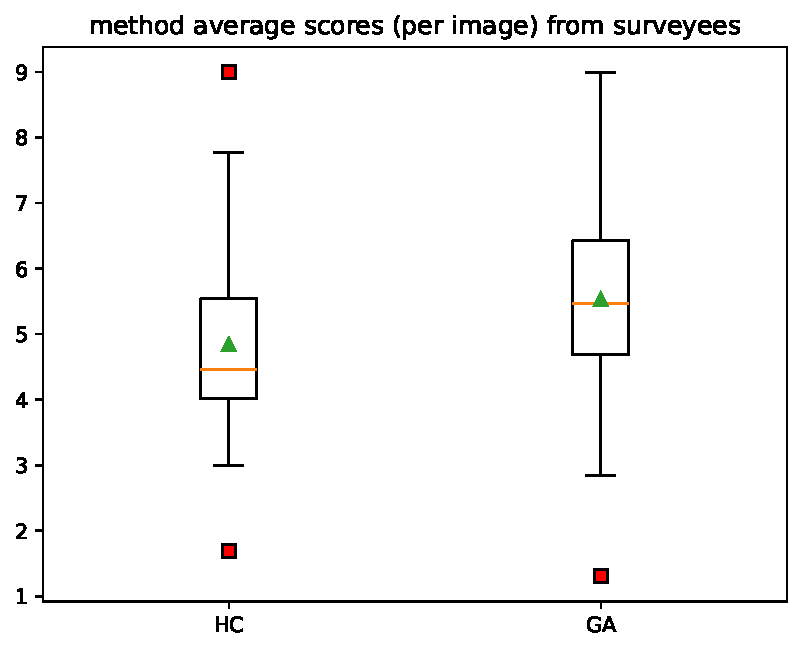
\includegraphics[width=\linewidth]{surveyee_score_box_plot.pdf}
  \caption{}
  \label{fig:survey_result_boxplot}
\end{subfigure}
  \caption{Average scores assigned to images enhanced by the HC and GA methods, as rated by survey participants  
  %Method $1$ represents Hill Climbing with neighborhood generation with split mutation (\ref{subsubsection:method_hc_traptri_split}) and method $2$ represents Genetic Algorithm with (P, P) strategy (see Section \ref{subsection:method_ga_join}) 
  }
  \label{fig:survey_result}
\end{figure}

From Figure \ref{fig:survey_result}, we can see the mean scores of all enhanced images given by each surveyee. 
Each data point in Figure \ref{fig:survey_result}(a) indicates the mean of scores given by one participant. Figure \ref{fig:survey_result}(b) shows the mean (triangle inside each box, green in color picture), and median (horizontal line inside each box, orange in color picture) of the responses. The red points are outliers according to the $1.5 \times$IQR rule \cite{rousseeuw2011robust}.
From Figure \ref{fig:survey_result}(a), GA shows a better mean score than HC (mean over participants). From Figure \ref{fig:survey_result}(b), we can see that HC has a higher chance of degrading the image (dense below score $5$), although GA has achieved the image with the lowest score according to one participant.

\begin{figure*}
  % one image
  \begin{subfigure}[b]{0.16\textwidth}%
    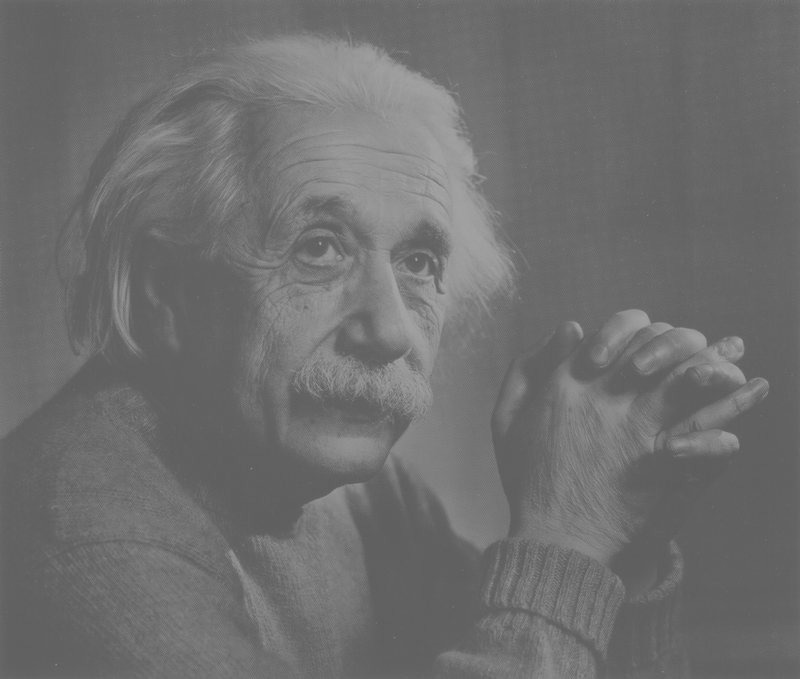
\includegraphics[width=\linewidth]{figures/original/07.jpg}
    \subcaption[]{Input}{}
    \label{fig:07_image_original}
  \end{subfigure}
  \begin{subfigure}[b]{0.16\textwidth}%
    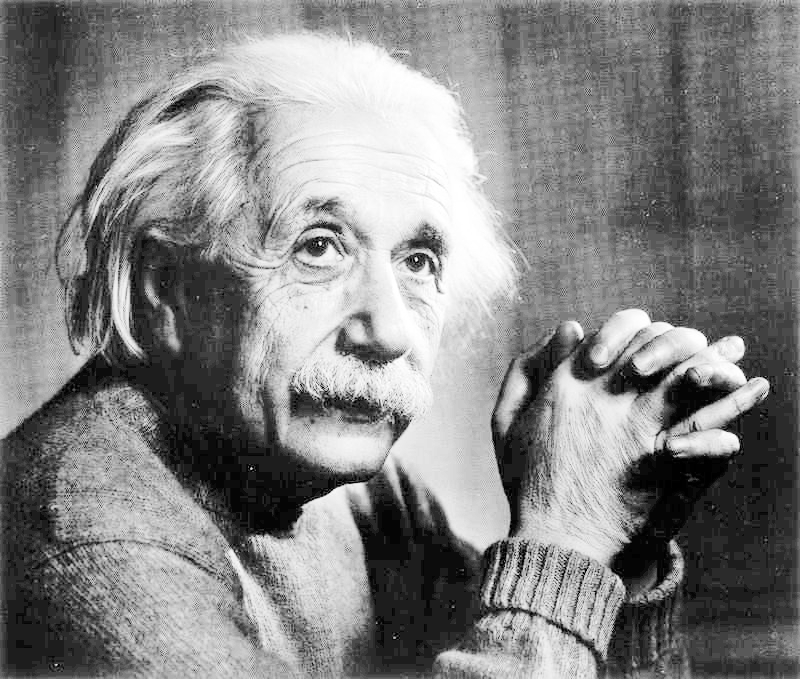
\includegraphics[width=\linewidth]{figures/he/07_output.jpg}
    \subcaption[]{HE}{}
    \label{fig:07_image_he}
  \end{subfigure}
  \begin{subfigure}[b]{0.16\textwidth}%
    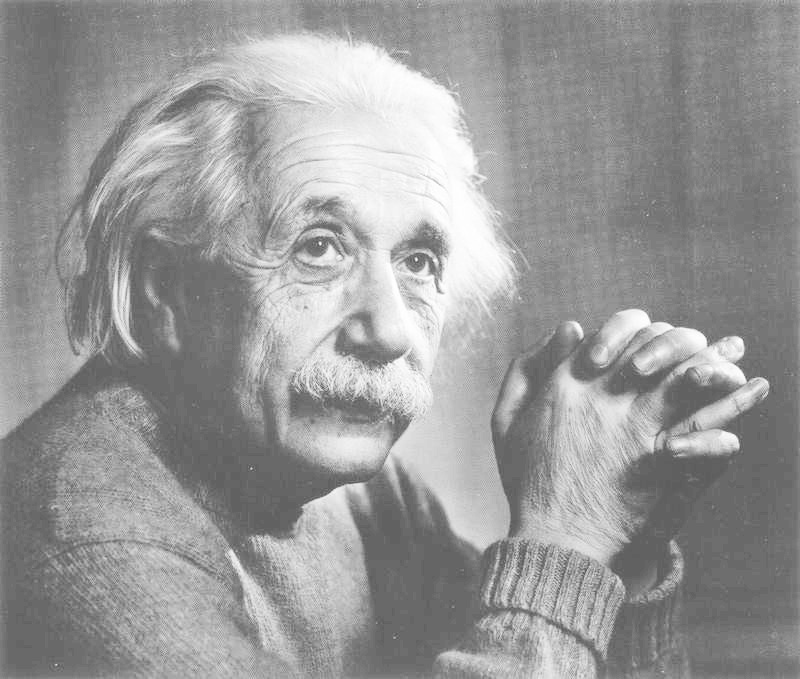
\includegraphics[width=\linewidth]{figures/agcwd/07_output.jpg}
    \subcaption[]{AGCWD}{}
    \label{fig:07_image_agcwd}
  \end{subfigure}
  \begin{subfigure}[b]{0.16\textwidth}%
    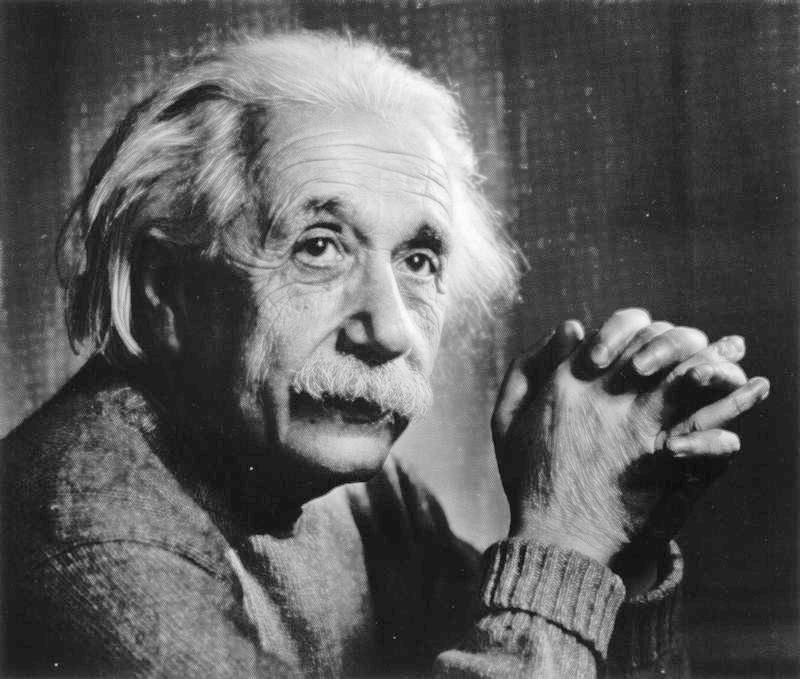
\includegraphics[width=\linewidth]{figures/dual/07_output.jpg}
    \subcaption[]{Dual}{}
    \label{fig:07_image_dual}
  \end{subfigure}
  \begin{subfigure}[b]{0.16\textwidth}%
    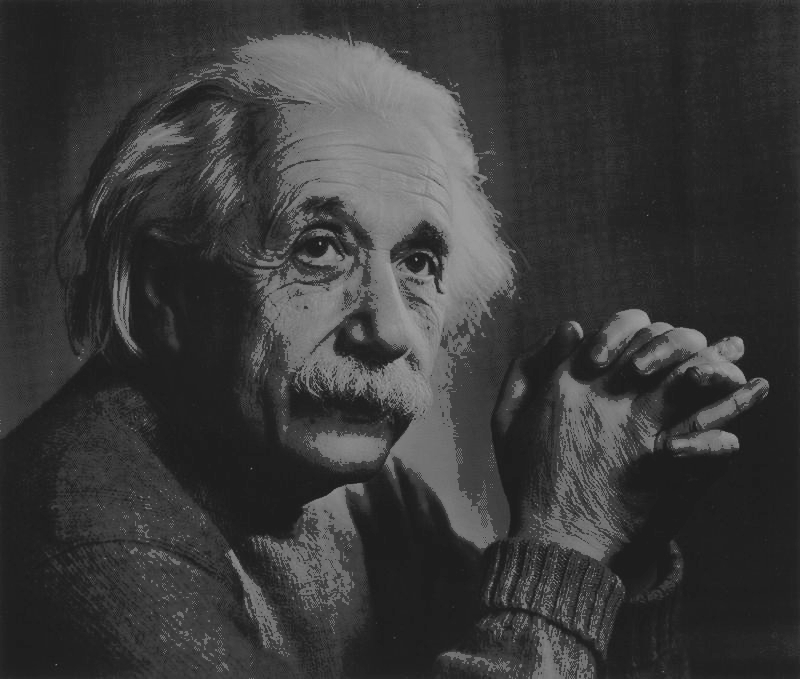
\includegraphics[width=\linewidth]{figures/hc_trap_split/07_output.jpg}
    \subcaption[]{HC}{}
    \label{fig:07_output_image_hc}
  \end{subfigure}
  \begin{subfigure}[b]{0.16\textwidth}%
    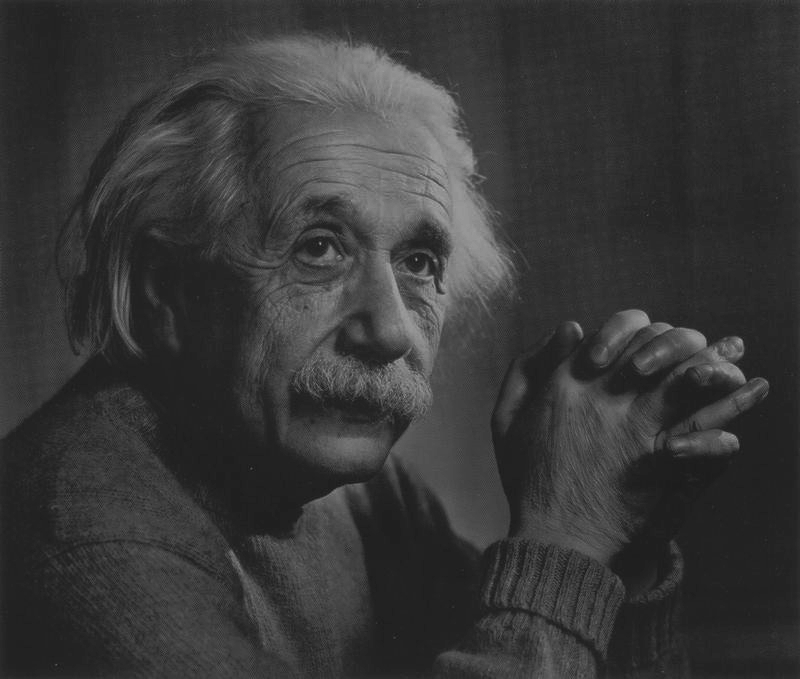
\includegraphics[width=\linewidth]{figures/ga_elitist/07_output.jpg}
    \subcaption[]{GA}{}
    \label{fig:07_output_image_ga}
  \end{subfigure}
  \vspace{-15pt}
  \caption{enhanced image generated by different techniques}
  \label{fig:07_result}
\end{figure*}
\begin{figure*}
  % one image
  % \begin{subfigure}[b]{0.33\textwidth}
  %   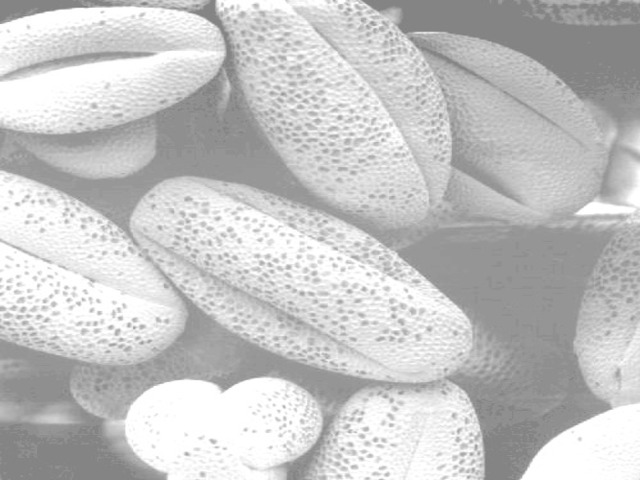
\includegraphics[width=\linewidth]{figures/original/08.jpg}
  %   \subcaption[]{}{}
  %   \label{fig:08_image_original}
  % \end{subfigure}
  % \begin{subfigure}[b]{0.33\textwidth}%
  %   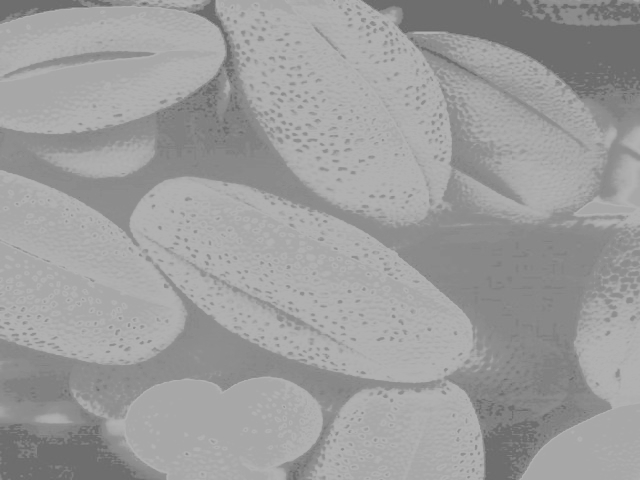
\includegraphics[width=\linewidth]{figures/hc_trap_split/08_output.jpg}
  %   \subcaption[]{}{}
  %   \label{fig:08_output_image_hc}
  % \end{subfigure}
  % \begin{subfigure}[b]{0.33\textwidth}%
  %   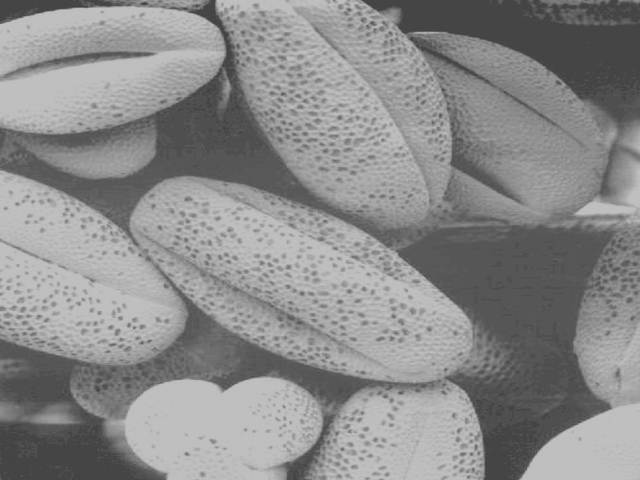
\includegraphics[width=\linewidth]{figures/ga_elitist/08_output.jpg}
  %   \subcaption[]{}{}
  %   \label{fig:08_output_image_ga}
  % \end{subfigure}
  % \vspace{-15pt}
  % \caption{enhanced image generated by different techniques}
  
  % \label{fig:08_result}

  % one image
  \begin{subfigure}[b]{0.16\textwidth}
    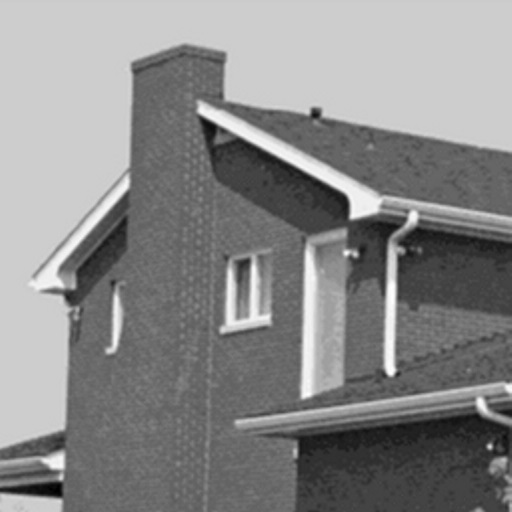
\includegraphics[width=\linewidth]{figures/original/house.jpg}
    \subcaption[]{Input}{}
    \label{fig:house_image_original}
  \end{subfigure}
  \begin{subfigure}[b]{0.16\textwidth}
    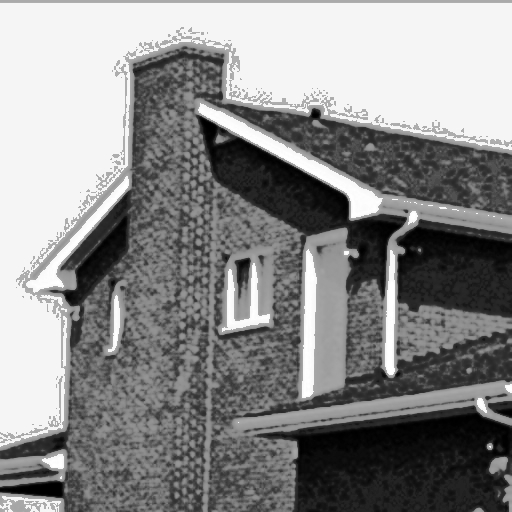
\includegraphics[width=\linewidth]{figures/he/house_output.jpg}
    \subcaption[]{HE}{}
    \label{fig:house_image_he}
  \end{subfigure}
  \begin{subfigure}[b]{0.16\textwidth}
    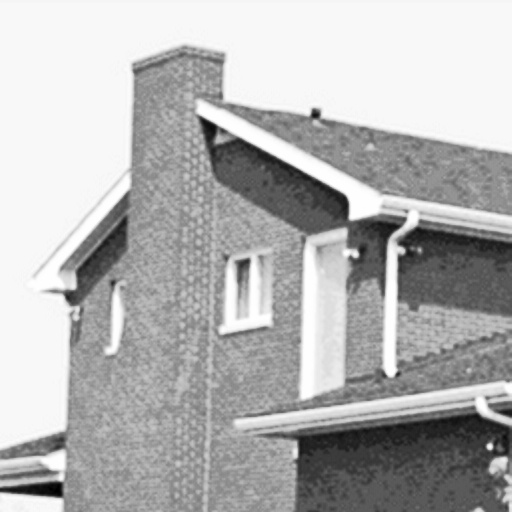
\includegraphics[width=\linewidth]{figures/agcwd/house_output.jpg}
    \subcaption[]{AGCWD}{}
    \label{fig:house_image_agcwd}
  \end{subfigure}
  \begin{subfigure}[b]{0.16\textwidth}
    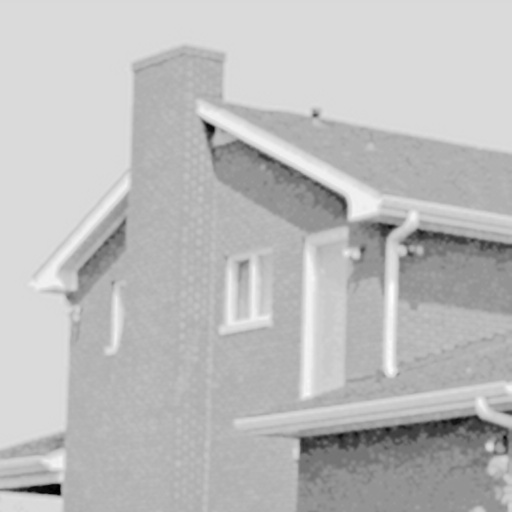
\includegraphics[width=\linewidth]{figures/dual/house_output.jpg}
    \subcaption[]{Dual}{}
    \label{fig:house_image_dual}
  \end{subfigure}
  \begin{subfigure}[b]{0.16\textwidth}%
    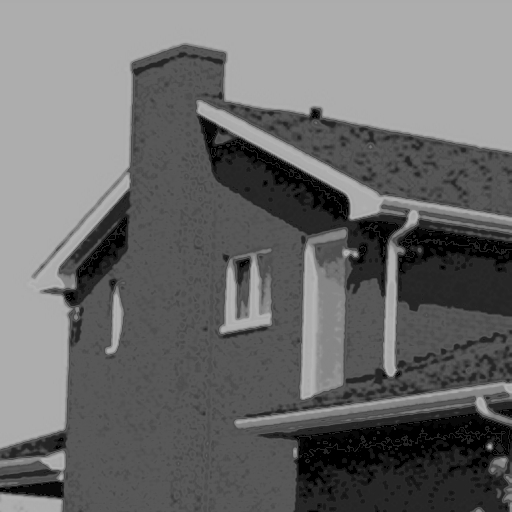
\includegraphics[width=\linewidth]{figures/hc_trap_split/house_output.jpg}
    \subcaption[]{HC}{}
    \label{fig:house_output_image_hc}
  \end{subfigure}
  \begin{subfigure}[b]{0.16\textwidth}%
    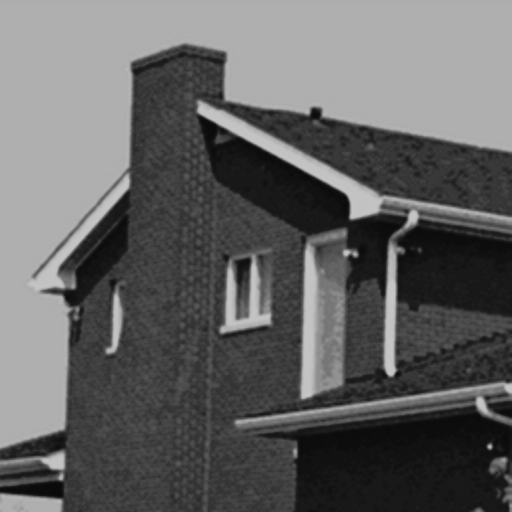
\includegraphics[width=\linewidth]{figures/ga_elitist/house_output.jpg}
    \subcaption[]{GA}{}
    \label{fig:house_output_image_ga}
  \end{subfigure}
  \vspace{-15pt}
  \caption{enhanced image generated by different techniques}
  \label{fig:house_result}
\end{figure*}
\begin{figure*}
  % one image
  \begin{subfigure}[b]{0.16\textwidth}
    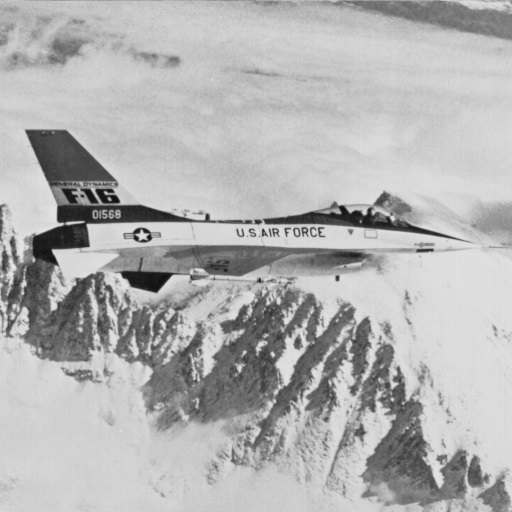
\includegraphics[width=\linewidth]{figures/original/jetplane.jpg}
    \subcaption[]{Input}{}
    \label{fig:jetplane_image_original}
  \end{subfigure}
  \begin{subfigure}[b]{0.16\textwidth}
    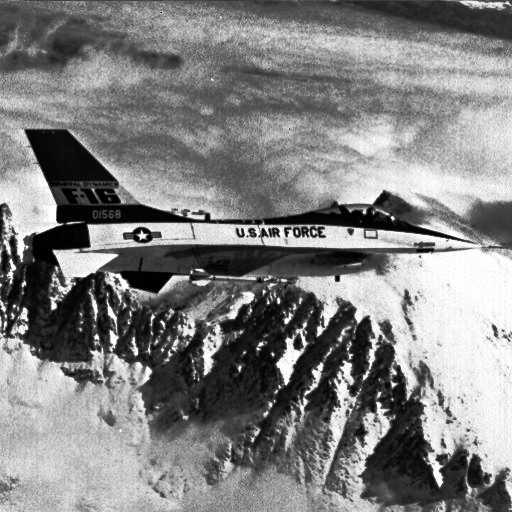
\includegraphics[width=\linewidth]{figures/he/jetplane_output.jpg}
    \subcaption[]{HE}{}
    \label{fig:jetplane_image_he}
  \end{subfigure}
  \begin{subfigure}[b]{0.16\textwidth}
    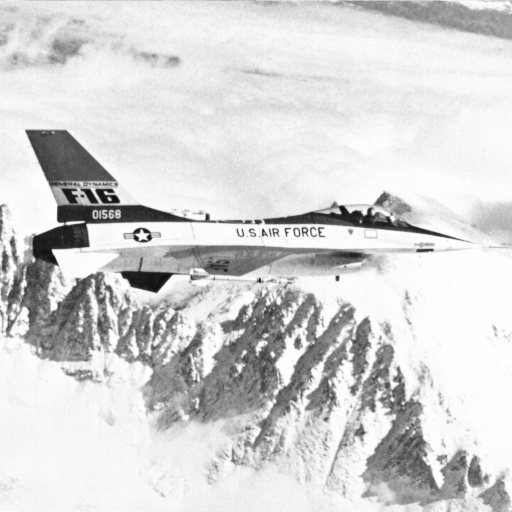
\includegraphics[width=\linewidth]{figures/agcwd/jetplane_output.jpg}
    \subcaption[]{AGCWD}{}
    \label{fig:jetplane_image_agcwd}
  \end{subfigure}
  \begin{subfigure}[b]{0.16\textwidth}
    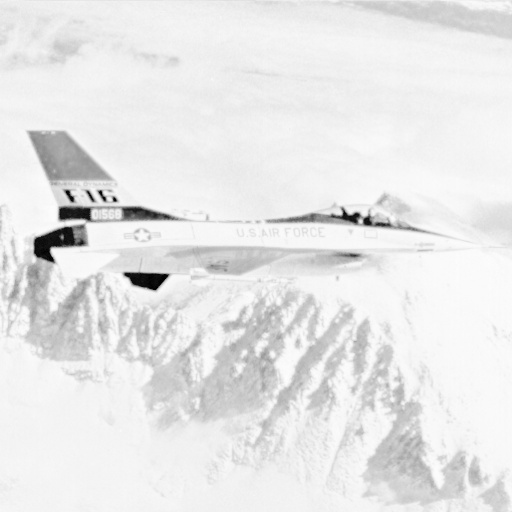
\includegraphics[width=\linewidth]{figures/dual/jetplane_output.jpg}
    \subcaption[]{Dual}{}
    \label{fig:jetplane_image_dual}
  \end{subfigure}
  \begin{subfigure}[b]{0.16\textwidth}%
    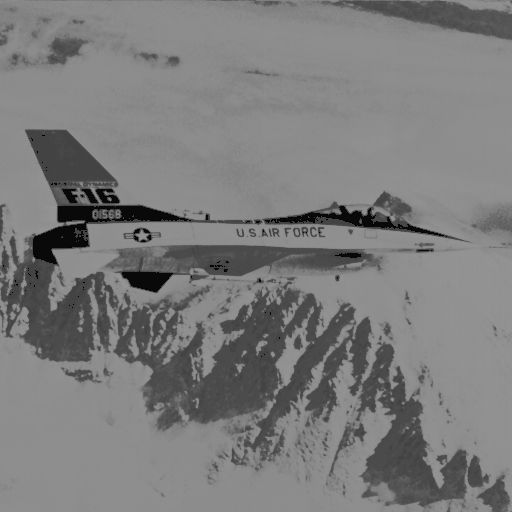
\includegraphics[width=\linewidth]{figures/hc_trap_split/jetplane_output.jpg}
    \subcaption[]{HC}{}
    \label{fig:jetplane_output_image_hc}
  \end{subfigure}
  \begin{subfigure}[b]{0.16\textwidth}%
    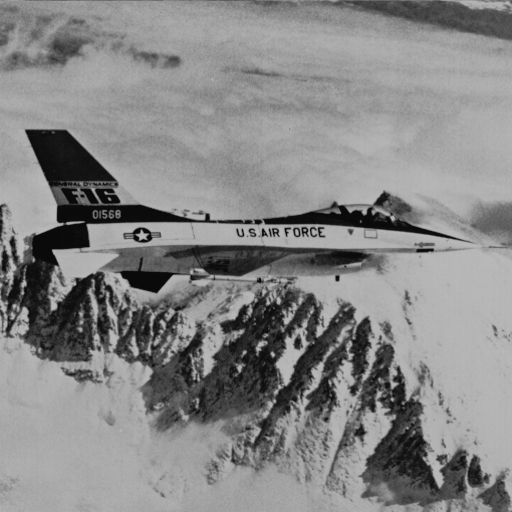
\includegraphics[width=\linewidth]{figures/ga_elitist/jetplane_output.jpg}
    \subcaption[]{GA}{}
    \label{fig:jetplane_output_image_ga}
  \end{subfigure}
  \vspace{-15pt}
  \caption{enhanced image generated by different techniques}
  \label{fig:jetplane_result}
\end{figure*}

% next page
\begin{figure*}
  % one image
  % \begin{subfigure}[b]{0.33\textwidth}
  %   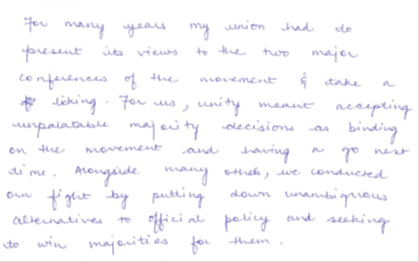
\includegraphics[width=\linewidth]{figures/original/11.png}
  %   \subcaption[]{}{}
  %   \label{fig:11_image_original}
  % \end{subfigure}
  % \begin{subfigure}[b]{0.33\textwidth}%
  %   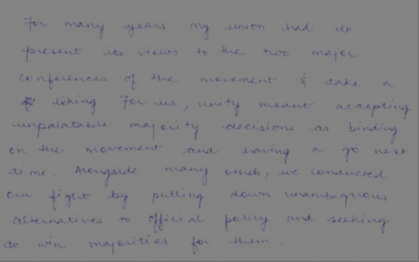
\includegraphics[width=\linewidth]{figures/hc_trap_split/11_output.jpg}
  %   \subcaption[]{}{}
  %   \label{fig:11_output_image_hc}
  % \end{subfigure}
  % \begin{subfigure}[b]{0.33\textwidth}%
  %   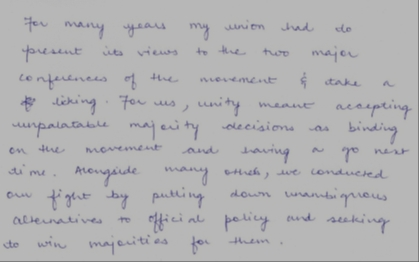
\includegraphics[width=\linewidth]{figures/ga_elitist/11_output.jpg}
  %   \subcaption[]{}{}
  %   \label{fig:11_output_image_ga}
  % \end{subfigure}
  % \caption{enhanced image generated by different techniques}
  % \label{fig:11_result}

  % one image
  % \begin{subfigure}[b]{0.33\textwidth}
  %   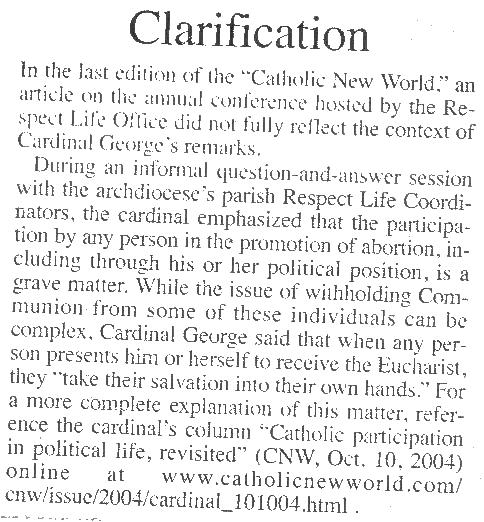
\includegraphics[width=\linewidth]{figures/original/12.jpg}
  %   \subcaption[]{}{}
  %   \label{fig:12_image_original}
  % \end{subfigure}
  % \begin{subfigure}[b]{0.33\textwidth}%
  %   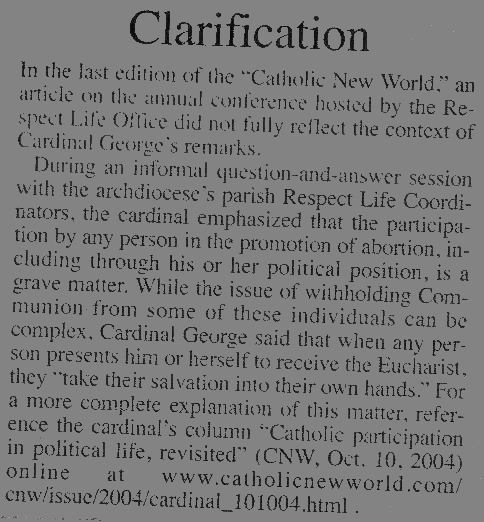
\includegraphics[width=\linewidth]{figures/hc_trap_split/12_output.jpg}
  %   \subcaption[]{}{}
  %   \label{fig:12_output_image_hc}
  % \end{subfigure}
  % \begin{subfigure}[b]{0.33\textwidth}%
  %   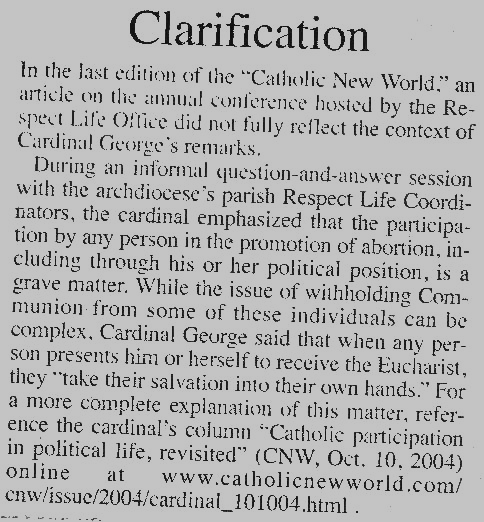
\includegraphics[width=\linewidth]{figures/ga_elitist/12_output.jpg}
  %   \subcaption[]{}{}
  %   \label{fig:12_output_image_ga}
  % \end{subfigure}
  % \caption{enhanced image generated by different techniques}
  % \label{fig:12_result}

  % one image
  \begin{subfigure}[b]{0.16\textwidth}
    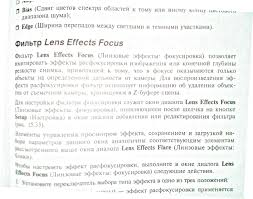
\includegraphics[width=\linewidth]{figures/original/13.jpg}
    \subcaption[]{Input}{}
    \label{fig:13_image_original}
  \end{subfigure}
  \begin{subfigure}[b]{0.16\textwidth}
    
\includegraphics[width=\linewidth]{figures/he/13_output.jpg}
    \subcaption[]{HE}{}
    \label{fig:13_image_he}
  \end{subfigure}
  \begin{subfigure}[b]{0.16\textwidth}
    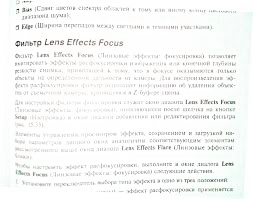
\includegraphics[width=\linewidth]{figures/agcwd/13_output.jpg}
    \subcaption[]{AGCWD}{}
    \label{fig:13_image_agcwd}
  \end{subfigure}
  \begin{subfigure}[b]{0.16\textwidth}
    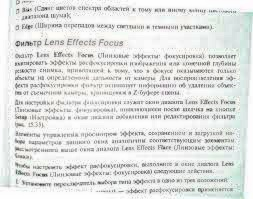
\includegraphics[width=\linewidth]{figures/dual/13_output.jpg}
    \subcaption[]{Dual}{}
    \label{fig:13_image_dual}
  \end{subfigure}
  \begin{subfigure}[b]{0.16\textwidth}%
    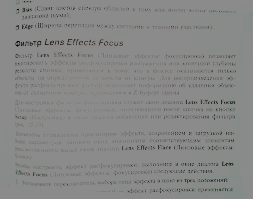
\includegraphics[width=\linewidth]{figures/hc_trap_split/13_output.jpg}
    \subcaption[]{HC}{}
    \label{fig:13_output_image_hc}
  \end{subfigure}
  \begin{subfigure}[b]{0.16\textwidth}%
    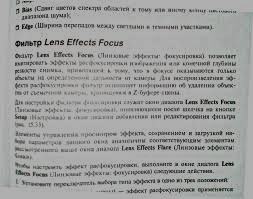
\includegraphics[width=\linewidth]{figures/ga_elitist/13_output.jpg}
    \subcaption[]{GA}{}
    \label{fig:13_output_image_ga}
  \end{subfigure}
  \caption{enhanced image generated by different techniques}
  \label{fig:13_result}
\end{figure*}
\begin{figure*}
  % one image
  % \begin{subfigure}[b]{0.33\textwidth}
  %   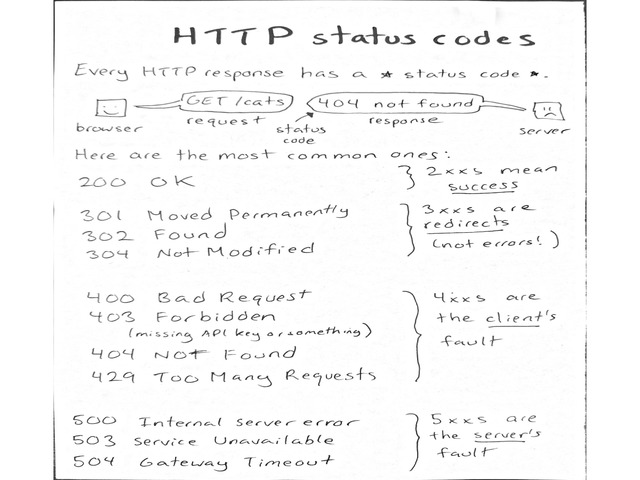
\includegraphics[width=\linewidth]{figures/original/09.jpg}
  %   \subcaption[]{}{}
  %   \label{fig:09_image_original}
  % \end{subfigure}
  % \begin{subfigure}[b]{0.33\textwidth}%
  %   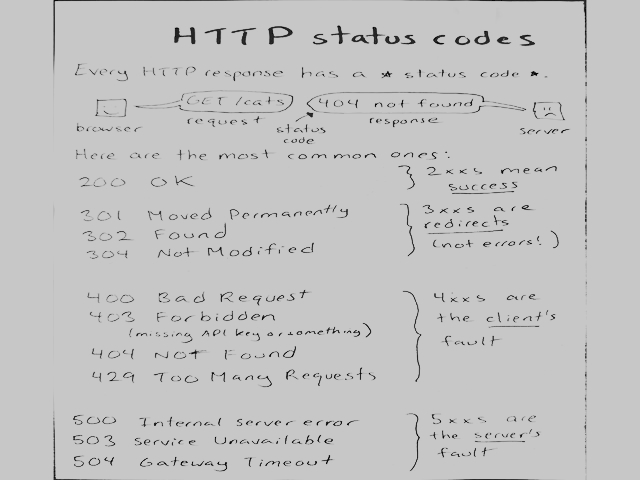
\includegraphics[width=\linewidth]{figures/hc_trap_split/09_output.jpg}
  %   \subcaption[]{}{}
  %   \label{fig:09_output_image_hc}
  % \end{subfigure}
  % \begin{subfigure}[b]{0.33\textwidth}%
  %   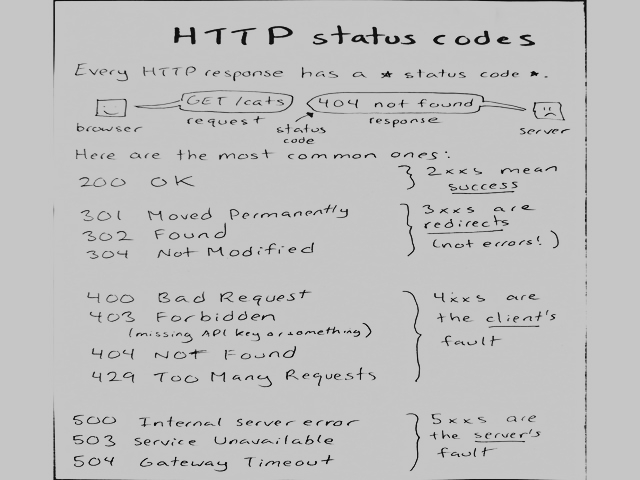
\includegraphics[width=\linewidth]{figures/ga_elitist/09_output.jpg}
  %   \subcaption[]{}{}
  %   \label{fig:09_output_image_ga}
  % \end{subfigure}
  % \caption{enhanced image generated by different techniques}
  % \label{fig:09_result}
% \end{figure*}

% next page
% \begin{figure*}
%   % one image
%   \begin{subfigure}[b]{0.33\textwidth}
%     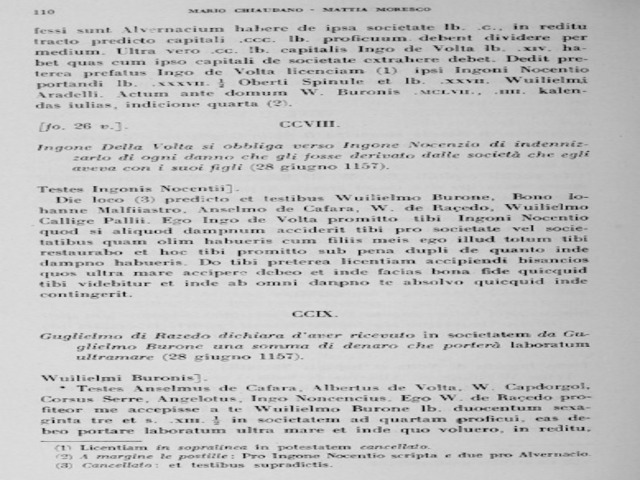
\includegraphics[width=\linewidth]{figures/original/10.jpg}
%     \subcaption[]{}{}
%     \label{fig:10_image_original}
%   \end{subfigure}
%   \begin{subfigure}[b]{0.33\textwidth}%
%     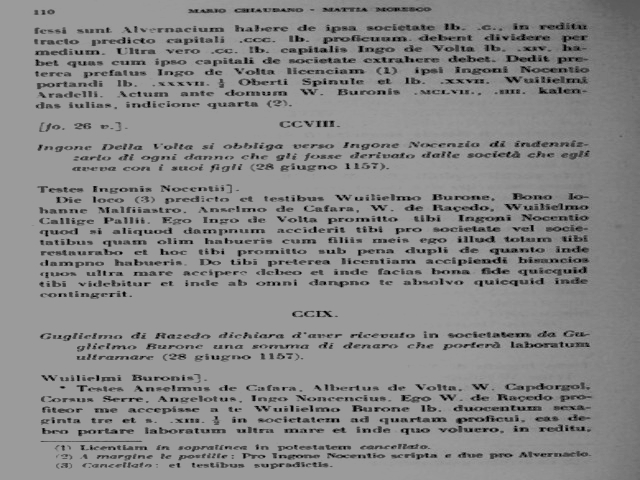
\includegraphics[width=\linewidth]{figures/hc_trap_split/10_output.jpg}
%     \subcaption[]{}{}
%     \label{fig:10_output_image_hc}
%   \end{subfigure}
%   \begin{subfigure}[b]{0.33\textwidth}%
%     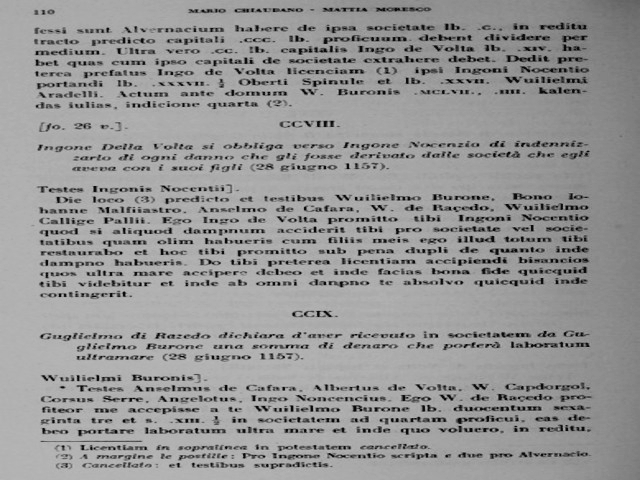
\includegraphics[width=\linewidth]{figures/ga_elitist/10_output.jpg}
%     \subcaption[]{}{}
%     \label{fig:10_output_image_ga}
%   \end{subfigure}
%   \caption{enhanced image generated by different techniques}
%   \label{fig:10_result}

%   % one image
%   \begin{subfigure}[b]{0.33\textwidth}
%     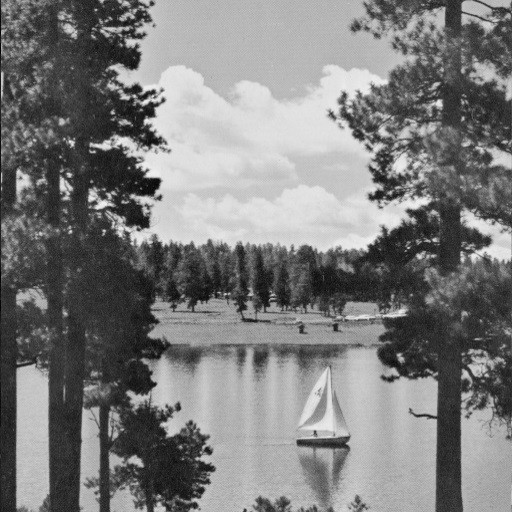
\includegraphics[width=\linewidth]{figures/original/lake.jpg}
%     \subcaption[]{}{}
%     \label{fig:lake_image_original}
%   \end{subfigure}
%   \begin{subfigure}[b]{0.33\textwidth}%
%     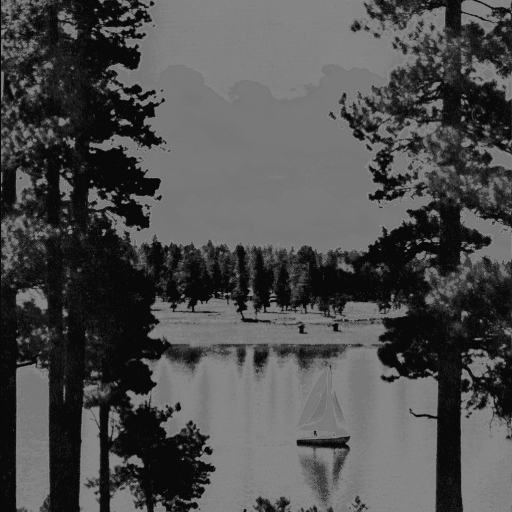
\includegraphics[width=\linewidth]{figures/hc_trap_split/lake_output.jpg}
%     \subcaption[]{}{}
%     \label{fig:lake_output_image_hc}
%   \end{subfigure}
%   \begin{subfigure}[b]{0.33\textwidth}%
%     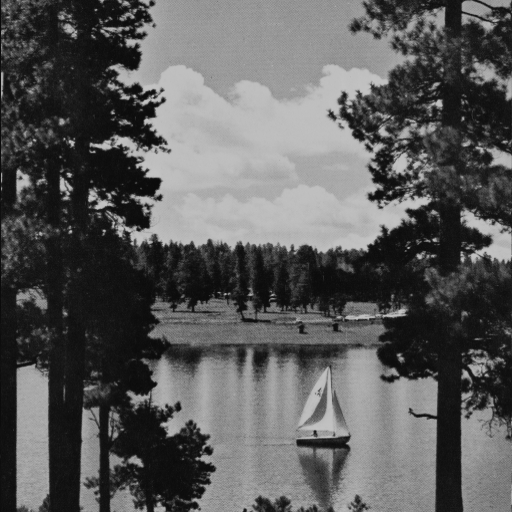
\includegraphics[width=\linewidth]{figures/ga_elitist/lake_output.jpg}
%     \subcaption[]{}{}
%     \label{fig:lake_output_image_ga}
%   \end{subfigure}
%   \caption{enhanced image generated by different techniques}
%   \label{fig:lake_result}

%   % one image
%   \begin{subfigure}[b]{0.33\textwidth}
%     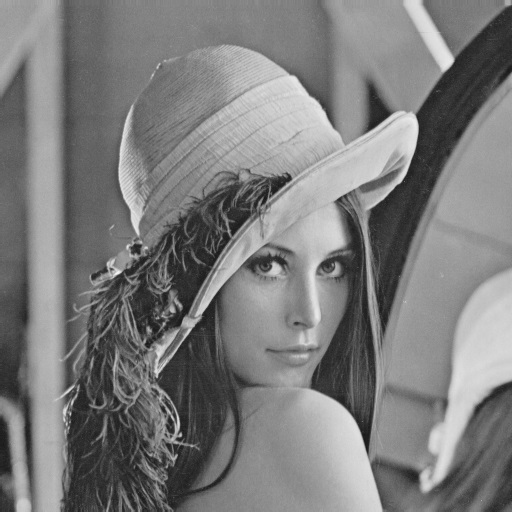
\includegraphics[width=\linewidth]{figures/original/lena_gray_512.jpg}
%     \subcaption[]{}{}
%     \label{fig:lenagray_image_original}
%   \end{subfigure}
%   \begin{subfigure}[b]{0.33\textwidth}%
%     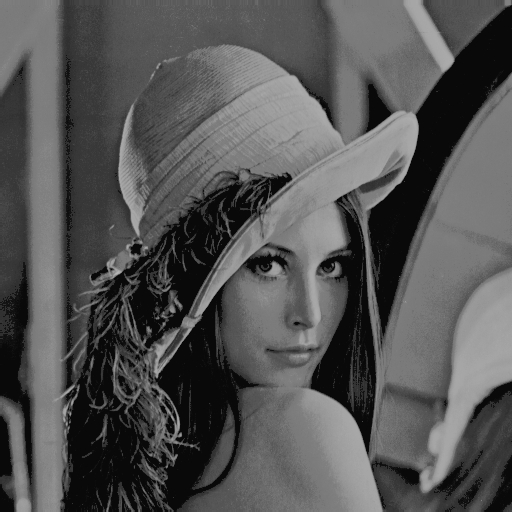
\includegraphics[width=\linewidth]{figures/hc_trap_split/lena_gray_512_output.jpg}
%     \subcaption[]{}{}
%     \label{fig:lenagray_output_image_hc}
%   \end{subfigure}
%   \begin{subfigure}[b]{0.33\textwidth}%
%     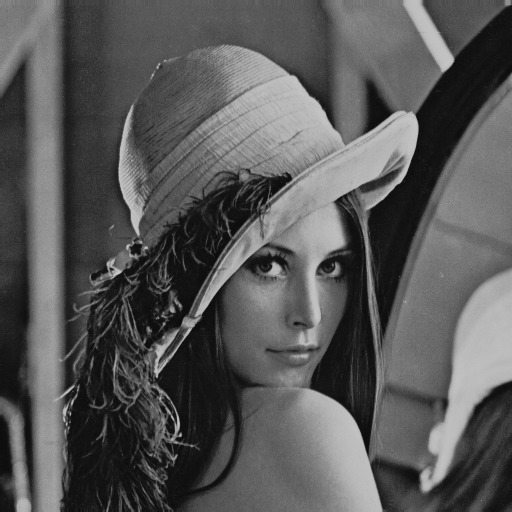
\includegraphics[width=\linewidth]{figures/ga_elitist/lena_gray_512_output.jpg}
%     \subcaption[]{}{}
%     \label{fig:lenagray_output_image_ga}
%   \end{subfigure}
%   \caption{enhanced image generated by different techniques}
%   \label{fig:lenagray_result}
% \end{figure*}

% next page
% \begin{figure*}
  % one image
  \begin{subfigure}[b]{0.16\textwidth}
    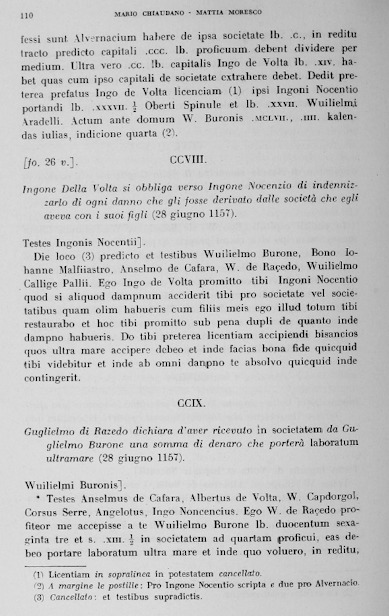
\includegraphics[width=\linewidth]{figures/original/06.jpg}
    \subcaption[]{Input}{}
    \label{fig:06_image_original}
  \end{subfigure}
  \begin{subfigure}[b]{0.16\textwidth}
    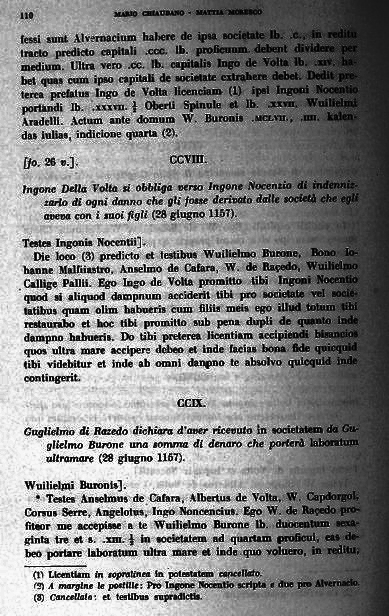
\includegraphics[width=\linewidth]{figures/he/06_output.jpg}
    \subcaption[]{HE}{}
    \label{fig:06_image_he}
  \end{subfigure}
  \begin{subfigure}[b]{0.16\textwidth}
    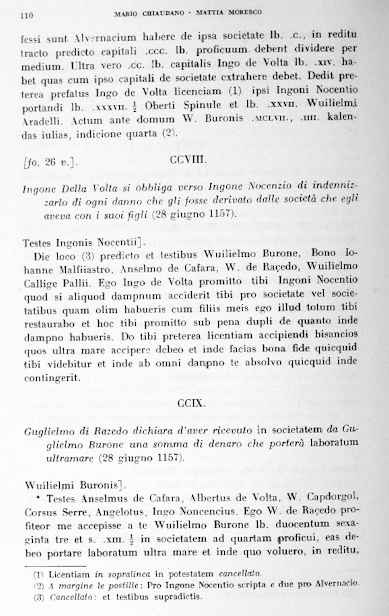
\includegraphics[width=\linewidth]{figures/agcwd/06_output.jpg}
    \subcaption[]{AGCWD}{}
    \label{fig:06_image_agcwd}
  \end{subfigure}
  \begin{subfigure}[b]{0.16\textwidth}
    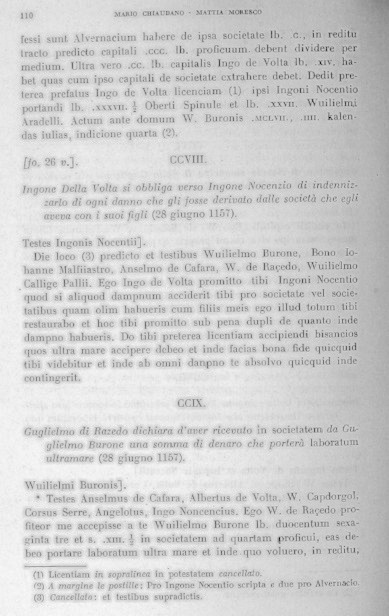
\includegraphics[width=\linewidth]{figures/dual/06_output.jpg}
    \subcaption[]{Dual}{}
    \label{fig:06_image_dual}
  \end{subfigure}
  \begin{subfigure}[b]{0.16\textwidth}%
    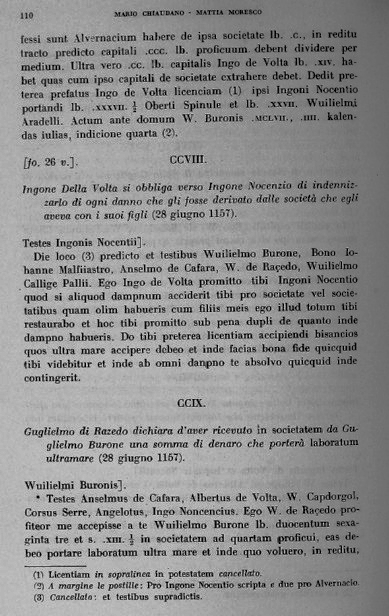
\includegraphics[width=\linewidth]{figures/hc_trap_split/06_output.jpg}
    \subcaption[]{HC}{}
    \label{fig:06_output_image_hc}
  \end{subfigure}
  \begin{subfigure}[b]{0.16\textwidth}%
    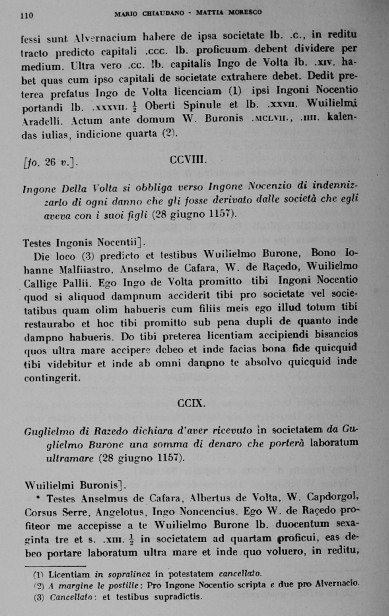
\includegraphics[width=\linewidth]{figures/ga_elitist/06_output.jpg}
    \subcaption[]{GA}{}
    \label{fig:06_output_image_ga}
  \end{subfigure}
  \caption{enhanced image generated by different techniques}
  \label{fig:06_result}
\end{figure*}
\begin{figure*}
  % one image
  \begin{subfigure}[b]{0.16\textwidth}
    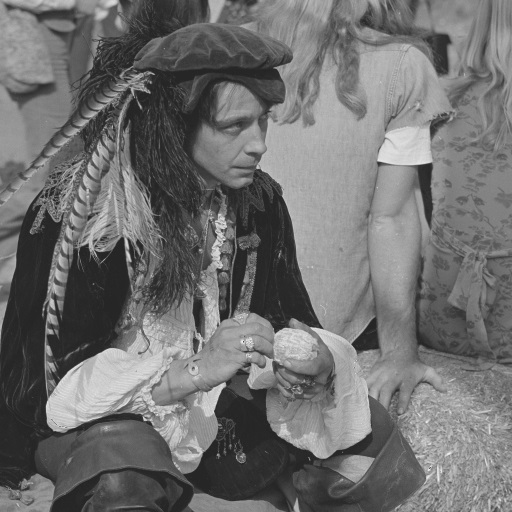
\includegraphics[width=\linewidth]{figures/original/pirate.jpg}
    \subcaption[]{Input}{}
    \label{fig:pirate_image_original}
  \end{subfigure}
  \begin{subfigure}[b]{0.16\textwidth}
    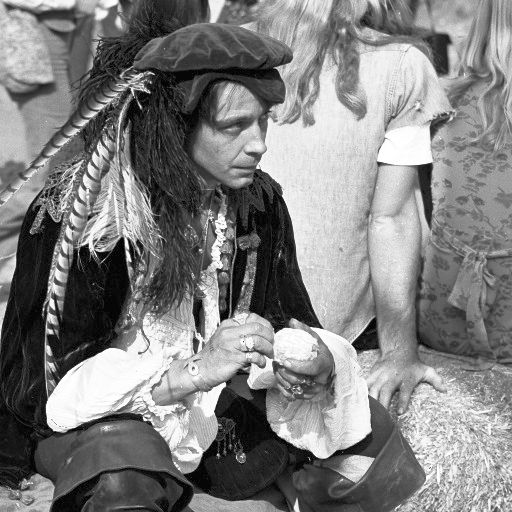
\includegraphics[width=\linewidth]{figures/he/pirate_output.jpg}
    \subcaption[]{HE}{}
    \label{fig:pirate_image_he}
  \end{subfigure}
  \begin{subfigure}[b]{0.16\textwidth}
    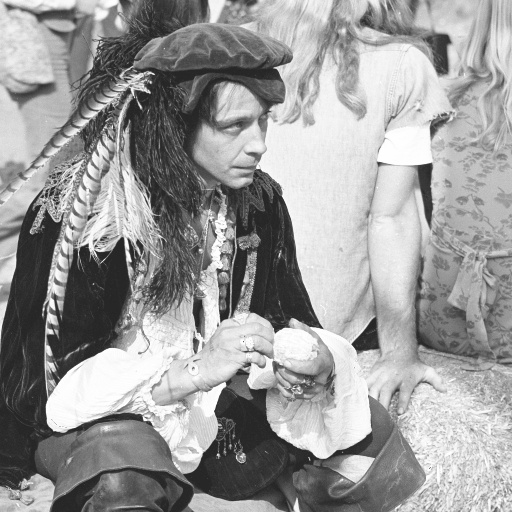
\includegraphics[width=\linewidth]{figures/agcwd/pirate_output.jpg}
    \subcaption[]{AGCWD}{}
    \label{fig:pirate_image_agcwd}
  \end{subfigure}
  \begin{subfigure}[b]{0.16\textwidth}
    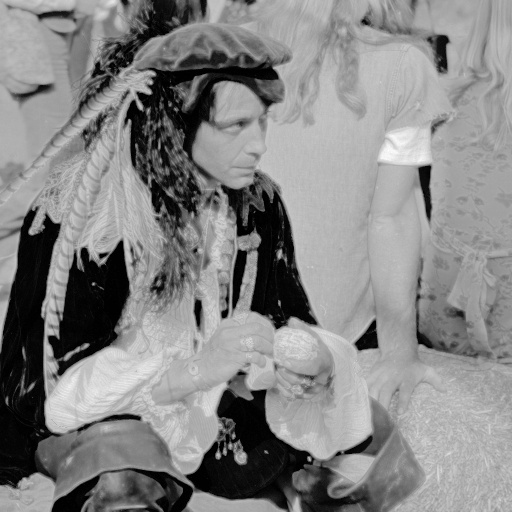
\includegraphics[width=\linewidth]{figures/dual/pirate_output.jpg}
    \subcaption[]{Dual}{}
    \label{fig:pirate_image_dual}
  \end{subfigure}
  \begin{subfigure}[b]{0.16\textwidth}%
    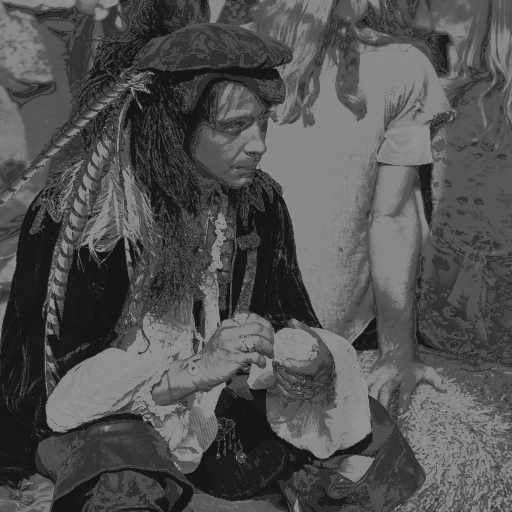
\includegraphics[width=\linewidth]{figures/hc_trap_split/pirate_output.jpg}
    \subcaption[]{HC}{}
    \label{fig:pirate_output_image_hc}
  \end{subfigure}
  \begin{subfigure}[b]{0.16\textwidth}%
    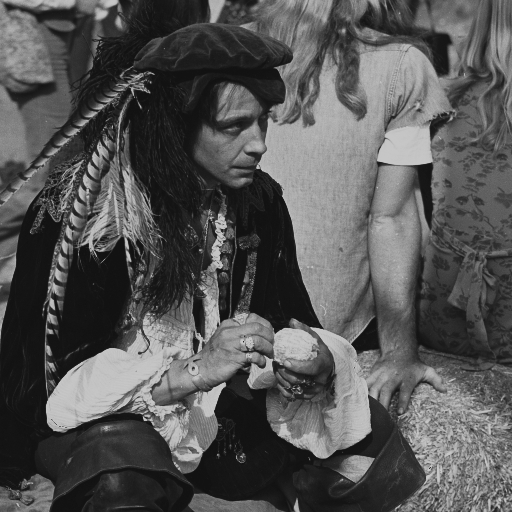
\includegraphics[width=\linewidth]{figures/ga_elitist/pirate_output.jpg}
    \subcaption[]{GA}{}
    \label{fig:pirate_output_image_ga}
  \end{subfigure}
  \caption{enhanced image generated by different techniques}
  \label{fig:pirate_result}
\end{figure*}
\begin{figure*}
  \begin{subfigure}[b]{0.16\textwidth}
    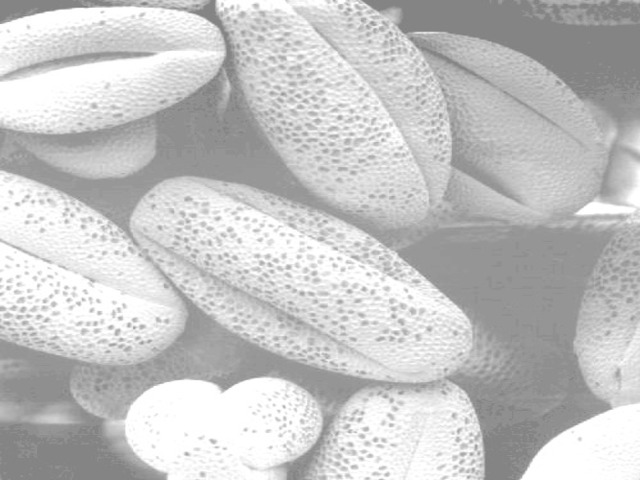
\includegraphics[width=\linewidth]{figures/original/08.jpg}
    \subcaption[]{Input}{}
    \label{fig:08_image_original}
  \end{subfigure}
  \begin{subfigure}[b]{0.16\textwidth}
    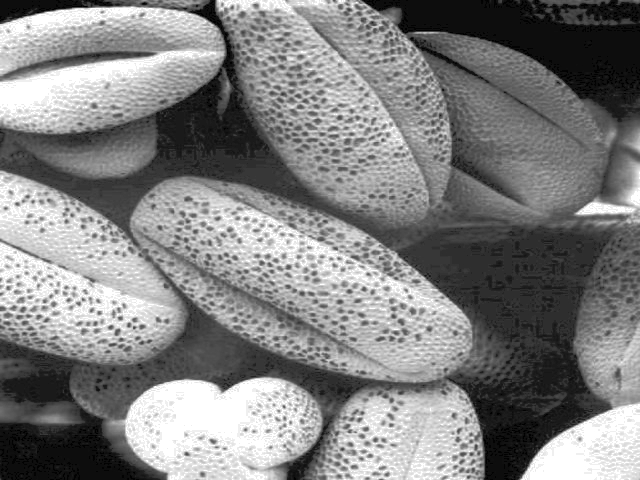
\includegraphics[width=\linewidth]{figures/he/08_output.jpg}
    \subcaption[]{HE}{}
    \label{fig:08_image_he}
  \end{subfigure}
  \begin{subfigure}[b]{0.16\textwidth}
    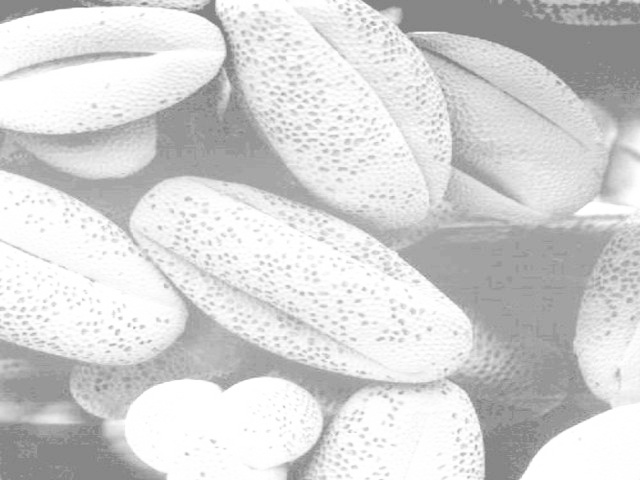
\includegraphics[width=\linewidth]{figures/agcwd/08_output.jpg}
    \subcaption[]{AGCWD}{}
    \label{fig:08_image_agcwd}
  \end{subfigure}
  \begin{subfigure}[b]{0.16\textwidth}
    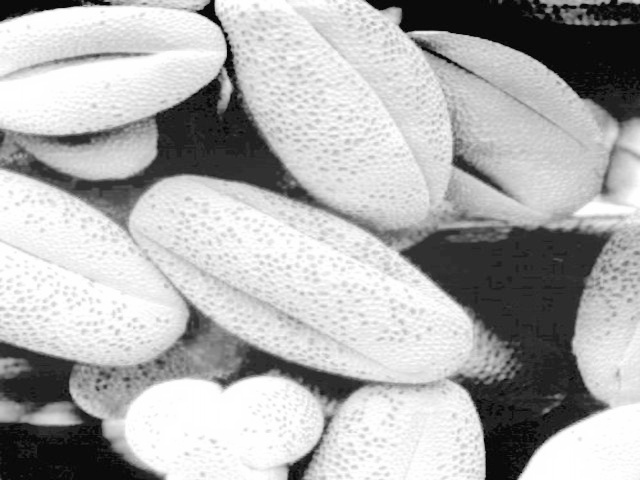
\includegraphics[width=\linewidth]{figures/dual/08_output.jpg}
    \subcaption[]{Dual}{}
    \label{fig:08_image_dual}
  \end{subfigure}
  \begin{subfigure}[b]{0.16\textwidth}%
    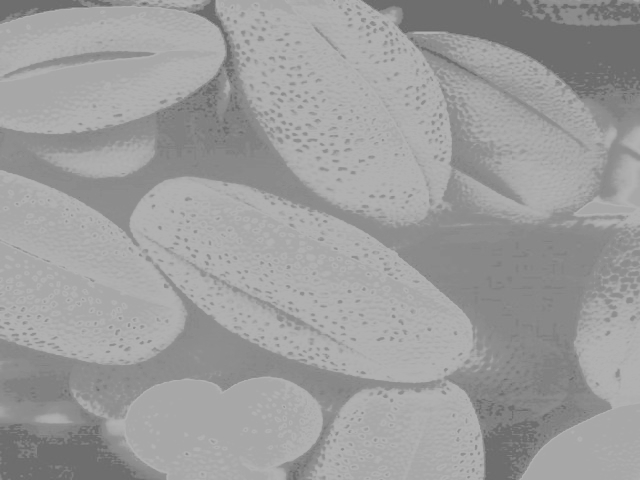
\includegraphics[width=\linewidth]{figures/hc_trap_split/08_output.jpg}
    \subcaption[]{HC}{}
    \label{fig:08_output_image_hc}
  \end{subfigure}
  \begin{subfigure}[b]{0.16\textwidth}%
    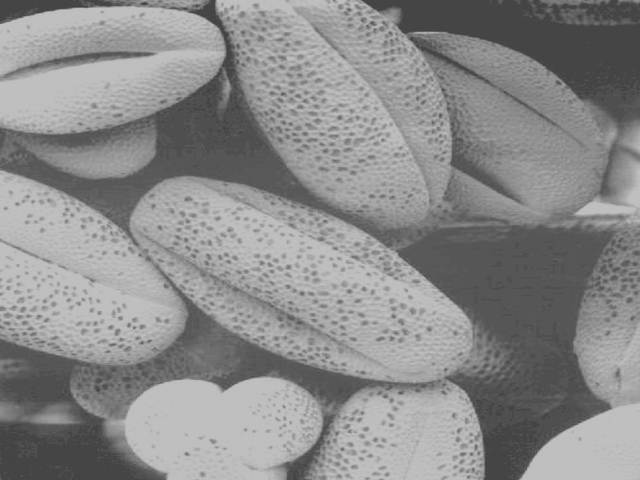
\includegraphics[width=\linewidth]{figures/ga_elitist/08_output.jpg}
    \subcaption[]{GA}{}
    \label{fig:08_output_image_ga}
  \end{subfigure}
  \vspace{-15pt}
  \caption{enhanced image generated by different techniques}
  
  \label{fig:08_result}
  
\end{figure*}

\begin{table*}[t]
    \centering
    \begin{tabular}{|c|c|c|c|c|c|c|c|c|c|c|c|c|c|c|c|c|}
        \hline
        \multirow{2}{8mm}{Image} & \multirow{2}{10mm}{Contrast} & \multicolumn{5}{|c|}{Contrast} & \multicolumn{5}{|c|}{PSNR} & \multicolumn{5}{|c|}{SSIM} \\
        \cline{3-17}
         & & HE & AGC & Dual & HC & GA & HE & AGC & Dual & HC & GA & HE & AGC & Dual & HC & GA \\
        \hline
          \Cref{fig:07_result} & 0.307 & 1.000 & 0.482 & 1.000 & 0.711 & 0.738 & 12.178 & 14.059 & 14.200 & 13.115 & 13.191 & 0.46 & 0.76 & 0.62 & 0.65 & 0.74\\
        \hline
          \Cref{fig:house_result} & 1.000 & 1.000 & 1.000 & 1.000 & 1.000 & 0.913 & 18.272 & 15.081 & 12.480 & 18.316 & 16.313 & 0.67 & 0.86 & 0.81 & 0.78 & 0.86\\
        \hline
          \Cref{fig:jetplane_result} & 0.894 & 1.000 & 0.889 & 1.000 & 1.000 & 0.909 & 12.077 & 17.231 & 12.559 & 12.967 & 15.260 & 0.55 & 0.96 & 0.79 & 0.84 & 0.9\\
        \hline
          \Cref{fig:13_result} & 0.802 & 1.000 & 0.802 & 1.000 & 0.893 & 0.903 & 6.322 & 31.501 & 22.375 & 7.553 & 9.689 & 0.29 & 0.95 & 0.89 & 0.61 & 0.89\\
        \hline
          \Cref{fig:06_result} & 1.000 & 1.000 & 1.000 & 1.000 & 1.000 & 0.912 & 9.554 & 18.066 & 21.031 & 13.239 & 15.925 & 0.52 & 0.98 & 0.84 & 0.88 & 0.95\\
        \hline
          \Cref{fig:pirate_result} & 0.774 & 1.000 & 0.752 & 1.000 & 0.791 & 0.843 & 18.220 & 14.389 & 17.006 & 17.681 & 18.644 & 0.87 & 0.87 & 0.72 & 0.76 & 0.83\\
        \hline
        \Cref{fig:08_result} & 0.339 & 1.000 & 1.000 & 1.000 & 0.262 & 0.500 & 10.598 & 22.720 & 13.632 & 14.787 & 12.978 & 0.67 & 0.93 & 0.77 & 0.69 & 0.91\\
        \hline
        \Cref{fig:11_result} & 0.360 & 1.000 & 0.360 & 0.727 & 0.320 & 0.399 & 7.442 & 41.648 & 33.793 & 6.510 & 11.110 & 0.3 & 0.99 & 0.98 & 0.7 & 0.94\\
        \hline
          \Cref{fig:12_result} & 0.917 & 1.000 & 1.000 & 1.000 & 0.908 & 0.903 & 8.438 & 27.879 & 16.463 & 6.850 & 13.004 & 0.48 & 0.97 & 0.63 & 0.69 & 0.94\\
        \hline
        \Cref{fig:09_result} & 1.000 & 1.000 & 1.000 & 1.000 & 0.923 & 0.913 & 6.845 & 33.446 & 22.716 & 13.545 & 13.161 & 0.24 & 0.98 & 0.88 & 0.93 & 0.95\\
        \hline
          \Cref{fig:10_result} & 0.925 & 1.000 & 0.931 & 1.000 & 0.902 & 0.909 & 9.614 & 17.897 & 15.826 & 12.781 & 14.873 & 0.53 & 0.98 & 0.79 & 0.91 & 0.95\\
        \hline
          \Cref{fig:lake_result} & 1.000 & 1.000 & 0.992 & 1.000 & 0.889 & 0.903 & 24.806 & 16.212 & 10.564 & 13.742 & 17.269 & 0.87 & 0.64 & 0.89 & 0.66 & 0.82\\
        \hline
          \Cref{fig:lenagray_result} & 0.836 & 1.000 & 0.821 & 1.000 & 0.916 & 0.886 & 19.460 & 14.725 & 12.843 & 16.009 & 16.740 & 0.88 & 0.88 & 0.76 & 0.79 & 0.84\\
        \hline
        \end{tabular}
    \caption{Michelson contrast, PSNR, and SSIM of proposed methods, histogram equalization (HE), dual channel (Dual), and adaptive gamma correction enhanced images (AGC), the contrast of reference image is in the second column. The image column contains the references to the input images.}
    \label{tab:image_metrics}
\end{table*}